\section{Frasortering af manglende data}
\label{TestAfSkalaSorteringAfData}
%
Testpersonernes respons på skalaerne omregnes til procent, hvorfor det venstre endepunkt er 0 \% og det højre endepunkt er 100 \%. Ud fra datasættet fremgår det, at nogle skalaer har én eller flere besvarelser på 0 \%, problemet med det er, at det ikke vides med sikkerhed om testpersonen har svaret 0 eller om testpersonen slet ikke har angivet en respons på den pågældende skala. At det ikke er muligt at adskille de to tilfælde fra hinanden skyldes, dels at programmet automatisk gemmer værdien 0 og ikke \textit{NaN}, hvis en skala ikke er besvaret og dels at det har været muligt at trykke \textit{Næste}, selvom der ikke er angivet en besvarelse. Det har derfor været nødvendigt at gennemgå datasættet og vurdere hver enkelte tilfælde i forhold til om det er en reel besvarelse eller om det er en manglende besvarelse. Dette afgøres på baggrund af to kriterier: 1) Hvis alle skalaerne, der er præsenteret på én af de syv sider, ikke er besvaret vil de alle være angivet med 0 i datasætte, hvorfor det kan fastslåes at det ikke er en reel besvarelse men derimod en manglende besvarelse. Årsagen til at der forekommer tilfælde, hvor en testperson ikke har besvaret en eneste skala på en af de præsenterede sider skyldes formentlig, at der har været problemer med programmet. Disse problemer relaterer sig hovedsageligt til \textit{Næste}-knappen i programmet, som reagerede dårligt og i nogle tilfælde kun ved dobbeltklik, så hvis en testperson klikkede flere gange på knappen er det muligt, at de sprang over en side og slet ikke blev præsenteret for de pågældende skalaer. 2) Hvis der ved en skala generelt er høje procentsatser og en besvarelse på 0 \% virker usandsynlig vil det betragtes som en manglende besvarelse. Er det tilfældet vil 0'et blive behandlet som en outlier, der er tre standard afvigelser fra det resterende data.\blankline
%
I henhold til datasættet, jævnfør \fullref{ElektroniskBilagExcel}, vil situationer, der opfylder kriterie 1) vedrørende manglende besvarelser, være markeret med en rød celle. Summeret forekommer det 16 gange, hvor største delen af fejlene er opstået på side syv, hvor hverken TP8, TP10, TP18, TP29, TP34 og TP36 har afgivet en besvarelse på hver af de fire præsenterede skalaer. \blankline
%
Der er 28 tilfælde hvor det er uvist hvorhvidt der enten er afgivet en besvarelse på 0 \% eller om 0 \% afspejler en manglende besvarelse. Dette vil blive undersøgt nærmere ved hjælp af nedenstående \autoref{fig:Boxplot0er}.
%
\begin{figure}[H]
\centering
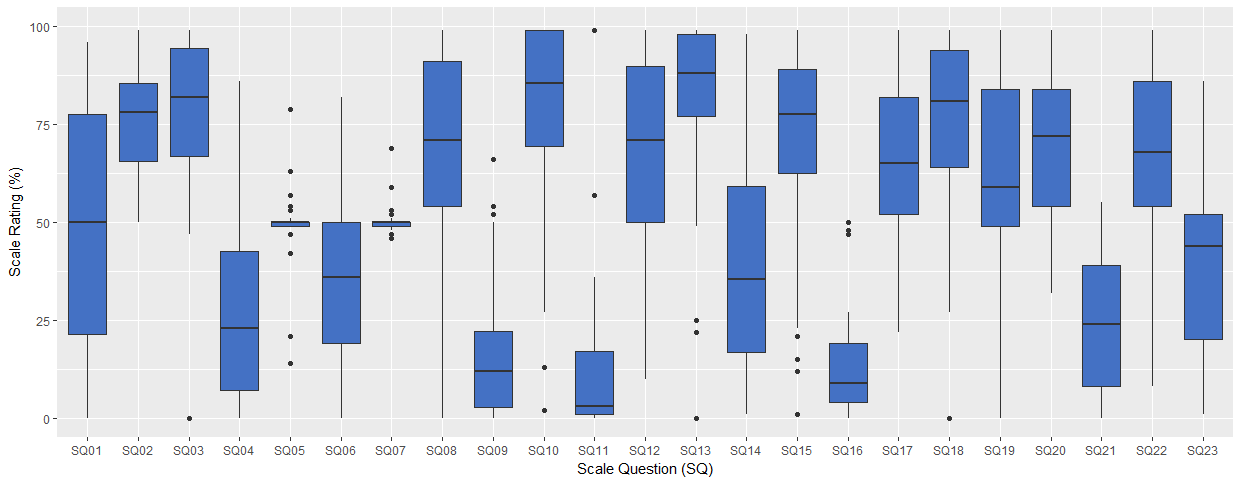
\includegraphics[width = \textwidth]{Figure/DatabehandlingSkalaer/BoksplotMed0er} 
\caption{Boksplot for besvarelserne på de 23 skalaer. Outliers er markeret med sorte prikker.}
\label{fig:Boxplot0er}
\end{figure}
\noindent
%
Boksplottet er lavet i \textit{RStudio}, hvor whiskers enten går fra den øverste eller nederste del af det interkvartile område til den største eller mindste værdi fundet 1.5 gang fra det interkvartile område, svarende til afstanden mellem første og tredje kvartil. Forefindes der et punkt udenfor disse whiskers betragtes det som en outlier.

Der tages udelukkende udgangspunkt i de outliers, der har værdien 0, hvilket er tilfældet for SQ3, SQ13 samt SQ18. Disse outliers er baseret på respons fra to testpersoner: TP18 til både SQ3 og SQ18, og TP30 til SQ13. Årsagen til at outlieren til SQ3, som vedrører hvor let det er at interagere med robotten, fjernes er, at den største grund til robotten sommetider kan være svær at interagere med skyldes skærmens reaktionsevne. Ved dette skala spørgsmål vurderede TP18, at skærmen reagerede 54 \% og der blev ydermere ikke observeret nogle problemer med interaktionen, som kunne indikere, at testpersonen havde oplevelsen af, at robotten var svær at interagere med. Det vurderes derfor, at det er usandsynligt, at testpersonen aktivt har svaret 0, men nærmere har været resultat af, at scalaprogrammet reagerede dårligt på input. Derfor eksluderes denne outlier. Den anden outlier, der forefindes i datasættet tilhørende TP18, er til SQ18, som vedrører hvor spændende robotten er. Baseret på observationer, hvor testpersonen virkede begejstret for mødet med robotten, samt besvarelsen til hvor glad testpersonen er for teknologi (91 \%) virker det usandsynligt at testpersonen har oplevet robotten som værende slet ikke spændende. Det vurderes derfor, at det er usandsyneligt at testpersonen aktivt har svaret 0, hvorfor denne outlier ekskluderes.

Den tredje outlier, som har værdien 0, forefindes ved SQ13, som vedrører hvorhvidt testpersonen stolede på at robotten fulgte en hen til det valgte sted. Hvis testpersonerne ved, hvor de skal hen, og robotten kører en anden vej, er der stor sandsynlighed for, at de ikke tror på at robotten kører det rigtige sted hen. Flere testpersoner gav udtryk for, at robotten kørte den forkerte vej, hvis de for eksempel skulle på toilettet og robotten kørte mod DutyFree. Derudover forekommer der to andre outliers til dette skala spørgsmål, jævnfør \autoref{fig:Boxplot0er}, hvor testpersonerne aktivt har svaret. Det vurderes derfor at der ikke er nok belæg for at ekskludere denne outlier. \blankline
%
De resterende outliers, der er forskellig fra 0, medtages alle da det er besvarelser testpersonerne aktivt har foretaget og derfor afspejler deres oplevelse af interaktionen med robotten.  
